%%%%%%%%%%%%%%%%%%%%%%
%%%%%%%%%%%%%%%%%%%%%%
%%Options for presentations (in-class) and handouts (e.g. print). 
%\documentclass[pdf]{beamer} 
\documentclass[pdf
%,handout
]{beamer}
%\usepackage{pgfpages}
%\pgfpagesuselayout{2 on 1}[letterpaper,border shrink=5mm]

%%%%%%%%%%%%%%%%%%%%%%
%% Change this for different slides so it appears in bar
\usepackage{authoraftertitle}
\date{Systems of Linear Equations}

%%%%%%%%%%%%%%%%%%%%%%
%% Upload common style file
\usepackage{../LyryxLinearAlgebraSlidesStyle}

\begin{document}

%%%%%%%%%%%%%%%%%%%%%%%
%% Title Page and Copyright Common to All Slides

%Title Page
\input ../frontmatter/titlepage.tex

%LOTS Page
%\input frontmatter/lyryxopentexts.tex

%Copyright Page
\input ../frontmatter/copyright.tex

%%%%%%%%%%%%%%%%%%%%%%%%%

\graphicspath{{../}}

\section{Systems of Linear Equations}

%-------------- start slide -------------------------------%
\frame{\frametitle{Motivation}

\begin{example} 
Solve 
\[
AX=B
\]
where $A\neq 0$. 
\pause

{\bf Solution} $X=B/A$. 
\pause

There are no other solutions; this is a unique solution. 
\end{example}


}
%-------------- end slide -------------------------------%

%------------------start slide ---------------------------%
\frame{\frametitle{Definitions}

A \emph{linear equation} is an expression
\[
a_1 x_1+a_2 x_2+\dots + a_n x_n = b
\]
where $n\geq 1$, $a_1,\dots, a_n$ are real numbers, \emph{not all of them equal to zero}, 
and $b$ is a real number. 
\pause
\medskip

A \emph{system of linear equations} is a set of $m\geq 1$ linear equations.  
It is not required that $m=n$. 
\pause
\medskip

\emph{Solution} to a system  of $m$ equations in  $n$ variables 
 is an $n$-tuple of numbers that satisfy each of the equations. 
\pause
\medskip

\emph{Solve a system} means `find \emph{all} solutions to the system.'
 
}
%-------------- end slide -------------------------------%

%-------------- start slide -------------------------------%
\frame{\frametitle{Systems of Linear Equations}
\begin{example}
A {\bf system} of {\bf linear equations}:
\[ \begin{array}{ccccccc}
x_1 & - & 2x_2 & - & 7x_3 & = & -1 \\
-x_1 & + & 3x_2 & + & 6x_3 & = & 0
\end{array}\]
\pause
\begin{itemize}
\item variables: $x_1$, $x_2$, $x_3$.
\pause
\item coefficients: 
\[ \begin{array}{ccccccc}
\alert{1}x_1 & - & \alert{2}x_2 & - & \alert{7}x_3 & = & -1 \\
\alert{-1}x_1 & + & \alert{3}x_2 & + & \alert{6}x_3 & = & 0
\end{array}\]
\pause
\item constant terms:
\[ \begin{array}{ccccccc}
x_1 & - & 2x_2 & - & 7x_3 & = & \alert{-1} \\
-x_1 & + & 3x_2 & + & 6x_3 & = & \alert{0}
\end{array}\]
\end{itemize}
\end{example}
}
%-------------- end slide -------------------------------%

%-------------- start slide -------------------------------%
\frame{
\begin{example}[continued]
$x_1= -3$, $x_2 = -1$, $x_3=0$ is a \alert{solution} to the system
\[ \begin{array}{ccccccc}
x_1 & - & 2x_2 & - & 7x_3 & = & -1 \\
-x_1 & + & 3x_2 & + & 6x_3 & = & 0
\end{array}\]
\pause
because
\[ \begin{array}{ccccccc}
(-3) & - & 2(-1) & - & 7 \cdot 0 & = & -1 \\
-(-3) & + & 3(-1) & + & 6\cdot 0 & = & 0. 
\end{array}\]
\pause
Another solution to the system is
$x_1= 6$, $x_2 = 0$, $x_3=1$ (check!).

\pause

However,
$x_1= -1$, $x_2 = 0$, $x_3=0$ \alert{is not} a solution to the
system, because
\[ \begin{array}{cccccccc}
(-1) & - & 2\cdot 0 & - & 7\cdot 0 & = & -1 \\
-(-1) & + & 3\cdot 0 & + & 6\cdot 0 & = & 1 & \neq 0
\end{array}\]

\pause

A {\bf solution to the system} must be a solution to {\bf every
equation} in the system.
\medskip

\pause
The system above is \alert{\bf consistent}, meaning that the system
has {\bf at least one} solution.
\end{example}
}
%-------------- end slide -------------------------------%

%-------------- start slide -------------------------------%
\frame{
\begin{example}[continued]
\[ \begin{array}{ccccccc}
x_1 & + & x_2 & + & x_3 & = & 0 \\
x_1 & + & x_2 & + & x_3 & = & -8
\end{array}\]
is an example of an \alert{\bf inconsistent} system,
meaning that it has no solutions.

\bigskip
\pause

\begin{center}
{\large Why are there no solutions?}
\end{center}
\bigskip

\end{example}
}
%-------------- end slide -------------------------------%

%------------------start slide ---------------------------%
\frame{\frametitle{Graphical Solutions}
\begin{example}
Consider the system of linear equations in two variables
\vspace*{-.15in}

\[ \begin{array}{c}
x+y=3 \\ y-x=5 \end{array}\]
\vspace*{-.15in}

\pause
A solution to this system is a pair $(x,y)$ satisfying both
equations.
\pause

Since each equation corresponds to a line, a solution to the
system corresponds to a point that lies on both lines, so the
solutions to the system can be found by graphing the two lines and
determining where they intersect.

\pause
\begin{picture}(3,1.35)
\put(1.25,0.1){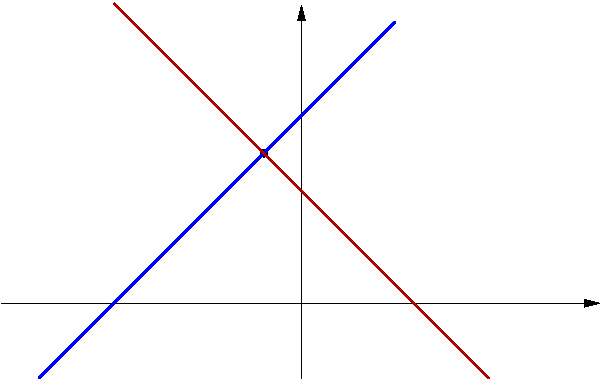
\includegraphics[scale=0.5]{figures/graph-soln.pdf}}
\textcolor{red}{
\put(1.2,1.1){\footnotesize{$x+y=3$}}}
\textcolor{blue}{
\put(2.5,1.1){\footnotesize{$y-x=5$}}}
\put(1.65,0.83){\scriptsize{$(-1,4)$}}
\end{picture}
\end{example} 
}
%---------------end slide----------------------------------%

%-------------- start slide -------------------------------%
\frame{
Given a system of two equations in two variables, 
graphed on the $xy$-coordinate plane, there
are three possibilities, as illustrated below.
\pause

\begin{picture}(4,2.0)
\put(0,0.5){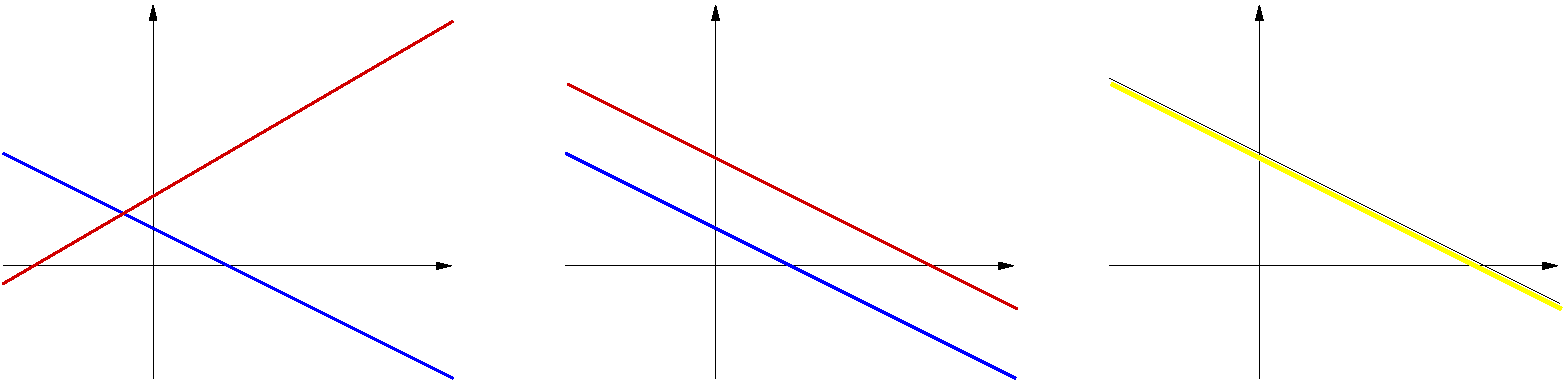
\includegraphics[scale=0.45]{figures/lines.pdf}}
\pause
\put(0.1,0.2){\footnotesize{intersect in one point}}
\pause
\put(0.1,0.0){\textcolor{red}{\footnotesize{consistent}}}
\put(0.1,-0.2){\footnotesize{(unique solution)}}
\pause
\put(1.8,0.2){\footnotesize{parallel but different}}
\pause
\put(1.8,0.0){\textcolor{red}{\footnotesize{inconsistent}}}
\put(1.8,-0.2){\footnotesize{(no solutions)}}
\pause
\put(3.4,0.2){\footnotesize{line are the same}}
\pause
\put(3.4,0.0){\textcolor{red}{\footnotesize{consistent}}}
\put(3.4,-0.2){\footnotesize{(infinitely many solutions)}}
\end{picture}
}
%---------------end slide----------------------------------%

%-------------- start slide -------------------------------%
\frame{
For a system of linear equations in {\bf two variables},
exactly one of the following holds:
\pause
\begin{enumerate}
\item the system is {\bf inconsistent};
\pause
\item the system has a {\bf unique} solution, i.e., exactly
one solution;
\pause
\item the system has {\bf infinitely many} solutions.
\end{enumerate}
\pause

(We will see in what follows that this generalizes to systems of
linear equations in more than two variables.)
}
%---------------end slide----------------------------------%

%-------------- start slide -------------------------------%
\frame{
\begin{example}
The system of linear equations in three variables that we saw
earlier
\[ \begin{array}{ccccccc}
x_1 & - & 2x_2 & - & 7x_3 & = & -1 \\
-x_1 & + & 3x_2 & + & 6x_3 & = & 0,
\end{array}\]
has solutions $x_1=-3+9s$, $x_2=-1+s$, $x_3=s$
where $s$ is any real number \alert{(written $s\in\RR$)}.
\pause

Verify this by substituting the expressions for $x_1$, $x_2$,
and $x_3$ into the two equations.

\pause

$s$ is called a \alert{parameter}, and the expression
\[
x_1=-3+9s, x_2=-1+s, x_3=s,~\mbox{where } s\in\RR\]

is called the
\alert{general solution} in parametric form.
\end{example}
}
%---------------end slide----------------------------------%

%-------------- start slide -------------------------------%
\frame{
\begin{problem}\em
Find all solutions to a system of $m$ linear equations in $n$
variables, i.e., \alert{solve a system of linear equations}.
\end{problem}

\pause
\begin{definition}
Two systems of linear equations are \alert{equivalent} if they
have {\bf exactly the same} solutions.
\end{definition}

\pause
\begin{example}
The two systems of linear equations
\[ \begin{array}{ccccc}
2x & + & y & = & 2 \\
3x &  &  & = & 3 
\end{array}
\hspace*{.25in}\mbox{ and } \hspace*{.25in}
\begin{array}{ccccc}
x & + & y & = & 1 \\
&  & y & = & 0 
\end{array}\]
are {\bf equivalent} because both systems have the
unique solution $x=1$, $y=0$.
\end{example}
}
%-------------- end slide -------------------------------%

\section{Elementary Operations}

%-------------- start slide -------------------------------%
\frame{\frametitle{Elementary Operations}

\begin{alertblock}{}
We solve a system of linear equations by using {\em Elementary Operations} 
to transform the system into an equivalent but simpler system from which 
the solution can be easily obtained.
\end{alertblock}
\pause

\begin{block}{Three types of Elementary Operations}
\pause
\begin{itemize}
\item {\bf Type I:} Interchange two equations,  \alert{$r_1\leftrightarrow r_2$}.
\pause
\item {\bf Type II:} Multiply an equation by a nonzero number, \alert{$13 r_1$}.
\pause
\item {\bf Type III:} 
Add a multiple of one equation to a different equation, \alert{$3r_3+r_2$}. 
\end{itemize}
\end{block}
}
%-------------- end slide -------------------------------%

%-------------- start slide -----------------------------%
\frame{\frametitle{Elementary Operations}

{\footnotesize
\begin{example}
Consider the system of linear equations
$\begin{array}{ccccccc}
3x_1 & - & 2x_2 & - & 7x_3 & = & -1 \\
-x_1 & + & 3x_2 & + & 6x_3 & = & 1\\
2x_1 &  &  & - & x_3 & = & 3
\end{array}$
\pause
\begin{itemize}
\item Interchange first two equations
(Type I elementary operation):
\[ 
\alert{r_1\leftrightarrow r_2}\qquad
\begin{array}{ccccccc}
-x_1 & + & 3x_2 & + & 6x_3 & = & 1\\
3x_1 & - & 2x_2 & - & 7x_3 & = & -1 \\
2x_1 &  &  & - & x_3 & = & 3
\end{array}\]
\vspace*{-.15in}

\pause
\item Multiply first equation by $-2$
(Type II elementary operation):
\[ \alert{-2r_1}\qquad 
\begin{array}{ccccccc}
-6x_1 & + & 4x_2 & + & 14x_3 & = & 2 \\
-x_1 & + & 3x_2 & + & 6x_3 & = & 1\\
2x_1 &  &  & - & x_3 & = & 3
\end{array}\]
\vspace*{-.15in}

\pause
\item Add 3 time the second equation to the first equation
(Type III elementary operation):

\vspace*{-.2in}
\[ \alert{3r_2+r_1}
\qquad
\begin{array}{ccccccc}
&  & 7x_2 & + & 11x_3 & = & 2 \\
-x_1 & + & 3x_2 & + & 6x_3 & = & 1\\
2x_1 &  &  & - & x_3 & = & 3
\end{array}\]
\end{itemize}
\end{example}
}}
%-------------- end slide -------------------------------%

%-------------- start slide -----------------------------%
\frame{
\begin{theorem}[Elementary Operations and Solutions]\em
If an elementary operation is performed on a system of linear
equations, the resulting system of linear equations is
equivalent to the original system.
(As a consequence, performing 
a sequence of elementary operations on a system
of linear equations results in an equivalent system of linear equations.)
\end{theorem}
}
%------------------ end slide ------------------------%

%--------------------start slide ---------------------%
\frame{\frametitle{Solving a System using Back Substitution}
\begin{problem}\em
Solve the system using back substitution
\[
\begin{array}{c}
2x+y = 4 \\
x - 3y = 1
\end{array}
\]
\end{problem}
\pause

\begin{solution}\em
Add $(-2)$ times the second equation to the first equation. 
\[
\begin{array}{c}
2x+y \alert{+ (-2)x - (-2)(3)y}= 4 \alert{+ (-2)1}\\
x - 3y = 1
\end{array}
\]
\pause
The result is an equivalent system
\[
\begin{array}{c}
7 y = 2 \\
x - 3y = 1
\end{array}
\]
\end{solution}
}
%------------------ end slide -----------------------%

%------------------start slide------------------%
\frame{
\begin{solution}[continued]\em
The first equation of the system,
\vspace*{-.15in}

\[
\alert{7y=2}
\]
\vspace*{-.25in}

can be rearranged to give us
\vspace*{-.15in}
\[
\alert{y= \frac{2}{7}}.
\]

\pause
Substituting $y=\frac{2}{7}$ into second equation:
\vspace*{-.15in}

\[
x - 3y = x - 3 \left(\alert{\frac{2}{7}}\right)= 1,
\]
\pause 
and simplifying, gives us
\vspace*{-.15in}

\[
x = 1 + \frac{6}{7} = \frac{13}{7}.
\]
\pause
Therefore, the solution is $x={13}/{7}, y = {2}/{7}$.
\pause
\bigskip

The method illustrated in this example is called \alert{back substitution.}
\end{solution}
We shall describe an \emph{algorithm} for solving any given system of linear equations.  
}
%-------------------end slide --------------------%

\section{Gaussian Elimination}

%-------------- start slide -------------------------------%
\frame{\frametitle{The Augmented Matrix}
Represent a system of linear equations with its
augmented matrix.
\begin{example}
The system of linear equations
\shiftup{0.5}
\[ \begin{array}{ccccccc}
x_1 & - & 2x_2 & - & 7x_3 & = & -1 \\
-x_1 & + & 3x_2 & + & 6x_3 & = & 0
\end{array}\]

\vspace*{-.1in}
is represented by the \alert{augmented matrix}
\shiftup{0.5}
\[ \left[\begin{array}{rrr|r}
1 & -2 & -7 & -1 \\
-1 & 3 & 6 & 0
\end{array}\right] \]

\vspace*{-.1in}
(A \alert{matrix} is a rectangular array of numbers.)

\medskip
\pause

{\bf Note.}
Two other \alert{matrices} associated with a system of
linear equations are the \textcolor{orange}{coefficient matrix} 
and the \textcolor{blue}{constant matrix}.
\[ \textcolor{orange}{\left[\begin{array}{rrr}
1 & -2 & -7\\ -1 & 3 & 6 \\
\end{array}\right]},~
\textcolor{blue}{\left[\begin{array}{r}
-1 \\ 0 \end{array}\right]}
\]
\end{example}
}
%-------------- end slide -------------------------------%

%-------------- start slide -------------------------------%
\frame{\frametitle{Elementary Row Operations}
For convenience, instead of performing {\bf elementary operations} on a system
of linear equations, perform corresponding 
\alert{elementary row operations} on the 
corresponding {\bf augmented matrix}.
\bigskip\bigskip

\pause{
{\bf Type I:} Interchange two rows.
\begin{example}
Interchange rows 1 and 3.
\[
\left[\begin{array}{rrrr|r}
\textcolor{blue}{2} & \textcolor{blue}{-1} & \textcolor{blue}{0} & \textcolor{blue}{5} & \textcolor{blue}{-3 }\\
-2 & 0 & 3 & 3 & -1 \\
\textcolor{red}{0} & \textcolor{red}{5} & \textcolor{red}{-6} & \textcolor{red}{1} & \textcolor{red}{0} \\
1 & -4 & 2 & 2 & 2 
\end{array}\right] 
\onslide<+->
\xrightarrow[]{r_1\leftrightarrow r_3}
\left[\begin{array}{rrrr|r}
\textcolor{red}{0} & \textcolor{red}{5} & \textcolor{red}{-6} & \textcolor{red}{1} & \textcolor{red}{0} \\
-2 & 0 & 3 & 3 & -1 \\
\textcolor{blue}{2} & \textcolor{blue}{-1} & \textcolor{blue}{0} & \textcolor{blue}{5} & \textcolor{blue}{-3} \\
1 & -4 & 2 & 2 & 2 
\end{array}\right]
\]
\end{example}}
}

%-------------- end slide -------------------------------%


%-------------- start slide -------------------------------%
\frame{\frametitle{Elementary Row Operations}
{\bf Type II:} Multiply a row by a nonzero number.
\begin{example}
Multiply row 4 by 2. 
\[
\left[\begin{array}{rrrr|r}
2 & -1 & 0 & 5 & -3 \\
-2 & 0 & 3 & 3 & -1 \\
0 & 5 & -6 & 1 & 0 \\
\textcolor{blue}{1} & \textcolor{blue}{-4} & \textcolor{blue}{2} & \textcolor{blue}{2} & \textcolor{blue}{2} 
\end{array}\right] 
\onslide<+->
\xrightarrow[]{2r_4}
\left[\begin{array}{rrrr|r}
2 & -1 & 0 & 5 & -3 \\
-2 & 0 & 3 & 3 & -1 \\
0 & 5 & -6 & 1 & 0 \\
\textcolor{blue}{2} & \textcolor{blue}{-8} & \textcolor{blue}{4} & \textcolor{blue}{4} & \textcolor{blue}{4} 
\end{array}\right]
\]
\end{example}
}
%-------------- end slide -------------------------------%

%-------------- start slide -------------------------------%
\frame{\frametitle{Elementary Row Operations}
{\bf Type III:}
Add a multiple of one row to a different row.
\begin{example} 
Add 2 times row 4 to row 2.
\[
\left[\begin{array}{rrrr|r}
2 & -1 & 0 & 5 & -3 \\
\textcolor{blue}{-2} & \textcolor{blue}{0} & \textcolor{blue}{3} & \textcolor{blue}{3} & \textcolor{blue}{-1} \\
0 & 5 & -6 & 1 & 0 \\
1 & -4 & 2 & 2 & 2 
\end{array}\right] 
\onslide<+->
\xrightarrow[]{2r_4+r_2}
\left[\begin{array}{rrrr|r}
2 & -1 & 0 & 5 & -3 \\
\textcolor{blue}{0} & \textcolor{blue}{-8} & \textcolor{blue}{7} & \textcolor{blue}{7} & \textcolor{blue}{3 }\\
0 & 5 & -6 & 1 & 0 \\
1 & -4 & 2 & 2 & 2 
\end{array}\right]
\]
\end{example}
}
%-------------- end slide -------------------------------%

%\frame{End of lecture for Friday, January 10, 2014}

%-------------- start slide -------------------------------%
\frame{
\begin{definition}
Two matrices $A$ and $B$ are \alert{row equivalent} (or simply
equivalent) if one can be obtained from the other by a 
sequence of \alert{elementary row operations}.
\end{definition}

\pause

\begin{problem}\em
 Prove that  $A$  can be obtained from $B$  by a 
sequence of elementary row operations if and only if $B$ can be 
obtained from $A$ by a sequence of elementary row operations. 

Prove that row equivalence is an equivalence relation. 
\end{problem} 
}

%-------------- end slide -------------------------------%


%-------------- start slide -------------------------------%
\frame{\frametitle{Row-Echelon Matrix}
\begin{itemize}
\item All rows consisting entirely of zeros are at the 
bottom.
\item The first nonzero entry in each nonzero row is a $1$
\\(called the {\bf leading 1} for that row).
\item Each leading 1 is to the right of all leading $1$'s 
in rows above it.
\end{itemize}
\begin{example}
\[
\left[\begin{array}{rrrrrrrr}
0 & 1 & * & * & * & * & * & * \\
0 & 0 & 0 & 1 & * & * & * & * \\
0 & 0 & 0 & 0 & 1 & * & * & * \\
0 & 0 & 0 & 0 & 0 & 0 & 0 & 1 \\
0 & 0 & 0 & 0 & 0 & 0 & 0 & 0 \\
0 & 0 & 0 & 0 & 0 & 0 & 0 & 0 
\end{array}\right] 
\]
where $*$ can be any number.
\end{example}
\pause

A matrix is said to be in the \emph{row-echelon form} (REF) if it is a row-echelon matrix. 
}
%-------------- end slide -------------------------------%


%-------------- start slide -------------------------------%
\frame{\frametitle{Reduced Row-Echelon Matrix}
\begin{itemize}
\item Row-echelon matrix.
\item Each leading 1 is the only nonzero entry in its
column.
\end{itemize}
\begin{example}
\[
\left[\begin{array}{rrrrrrrr}
0 & 1 & * & 0 & 0 & * & * & 0 \\
0 & 0 & 0 & 1 & 0 & * & * & 0 \\
0 & 0 & 0 & 0 & 1 & * & * & 0 \\
0 & 0 & 0 & 0 & 0 & 0 & 0 & 1 \\
0 & 0 & 0 & 0 & 0 & 0 & 0 & 0 \\
0 & 0 & 0 & 0 & 0 & 0 & 0 & 0 
\end{array}\right] 
\]
where $*$ can be any number.
\end{example}
\pause

A matrix is said to be in the  \emph{reduced row-echelon form} (RREF) if it is a reduced row-echelon matrix. 


}
%-------------- end slide -------------------------------%

%-------------- start slide -------------------------------%
\frame{\frametitle{Examples}

Which of the following matrices are in the REF? 

\medskip

Which ones are in the RREF?  

\medskip
\pause

(a) $\left[ \begin{array}{rrrr}  0 & 1 & 2 & 0\\ 0 & 0 & 1 & 2 \end{array}\right]$, 
(b) $\left[ \begin{array}{rrrr}   1 & 0 & 2 & 0\\ 0 & 0 & 1 & 2 \end{array}\right]$, 
(c) $\left[ \begin{array}{rrrr}  1 & 0 & 2 & 0\\ 0 & 0 & 1 & 2\\0 & 0 & 1 & 2 \end{array}\right]$

(d) $\left[ \begin{array}{rrrr}   1 & 0 & 2 & 0\\ 0 & 1 & 1 & 2 \end{array}\right]$, 
(e) $\left[ \begin{array}{rrrr}   1 & 2 & 0 & 0\\ 0 & 0 & 1 & 2 \end{array}\right]$, 
(f) $\left[ \begin{array}{rrrr}   1 & 2 & 0 & 0\\ 0 & 0 & 1 & 0\\0 & 0 & 0 & 1 \end{array}\right]$, 


}
%-------------- end slide -------------------------------%

%-------------- start slide -------------------------------%
\frame{
\begin{example}
Suppose that the following matrix is the augmented matrix 
of a system of linear equations.
We see from this matrix that the system of linear equations has
four equations and seven variables. 
\[ \left[\begin{array}{rrrrrrr|r}
\alert{1} & -3 & 4 & -2 & 5 & -7 & 0 & 4 \\
0 &  0 & \alert{1} &  8 & 0 & 3 & -7 & 0 \\
0 &  0 & 0 &  \alert{1} & 1 & -1 & 0 & -1 \\
0 &  0 & 0 &  0 & 0 & 0 & \alert{1} & 2 
\end{array}\right] \]
Note that the matrix is a \alert{row-echelon matrix}.
\pause
\begin{itemize}
\item Each column of the matrix corresponds to a variable, 
and the \alert{leading variables} are the variables that correspond
to columns containing leading ones
(in this case, columns 1, 3, 4, and 7).
\pause
\item The remaining variables (corresponding to columns 2, 5 and 6)
are called \alert{non-leading variables}.
\end{itemize}
\end{example}
\pause
We will use elementary row operations to transform a matrix to
row-echelon (REF) or reduced row-echelon form (RREF).
}
%-------------- end slide -------------------------------%

%-------------- start slide -------------------------------%
\frame{\frametitle{Solving Systems of Linear Equations}

\begin{alertblock}{}
``Solving a system of linear equations'' \textbf{means} 
finding {\bf all} solutions to the system.
\end{alertblock}
\pause
\bigskip

\begin{block}{\textbf{Method I: Gauss-Jordan Elimination}}

\begin{enumerate} 
\item Use elementary row operations to transform the augmented matrix
to an equivalent ({\bf not equal}) \alert{reduced row-echelon}
matrix.
The procedure for doing this is called the
\alert{Gaussian Algorithm}, or the
\alert{Reduced Row-Echelon Form Algorithm}.
\pause
\item If a row of the form $[0\;0\; \cdots 0\; | \; 1]$ occurs,
then there is no solution to the system of equations.
\pause
\item Otherwise assign \alert{parameters} to the 
\alert{non-leading variables}
(if any), and solve for the \alert{leading variables}
in terms of the parameters. 
\end{enumerate}
\end{block}
}
%-------------- end slide -------------------------------%


%-------------- start slide -------------------------------%
{\small
\frame{\frametitle{Gauss-Jordan Elimination}
\shiftup{0.5}
\begin{problem}\em
Solve the system
\vspace*{-.35in}

\[ \begin{array}{ccccccc}
2x & + & y & + & 3z & = & 1 \\
2y & - & z & + & x & = & 0 \\
9z & + & x & - & 4y & = & 2 
\end{array}\]
\end{problem}
\shiftup{0.5} 

\onslide<2->
\begin{solution}\em
\[
\left[\begin{array}{rrr|r}
2 & 1 & 3 & 1 \\
1 & 2 & -1 & 0 \\
1 & -4 & 9 & 2
\end{array}\right] 
\onslide<3->
\xrightarrow[]{r_1\leftrightarrow r_2}
\left[\begin{array}{rrr|r}
1 & 2 & -1 & 0 \\
2 & 1 & 3 & 1 \\
1 & -4 & 9 & 2
\end{array}\right] 
\]
\onslide<4->
\shiftup{0.5}
\[
%\xrightarrow[]{-2r_1+r_2, -r_1+r_3}
\xrightarrow[-2r_1+r_2]{-r_1+r_3}
\left[\begin{array}{rrr|r}
1 & 2 & -1 & 0 \\
0 & -3 & 5 & 1 \\
0 & -6 & 10 & 2
\end{array}\right] 
\onslide<5->
\xrightarrow[]{-r_2+r_3}
\left[\begin{array}{rrr|r}
1 & 2 & -1 & 0 \\
0 & -3 & 5 & 1 \\
0 & 0 & 0 & 0
\end{array}\right] 
\]
\shiftup{0.5}
\[
\onslide<6->
\xrightarrow[]{-\frac 13 r_2}
\left[\begin{array}{rrr|r}
1 & 2 & -1 & 0 \\
0 & 1 & -\vspace{0.05in}\frac{5}{3} & -\vspace{0.05in}\frac{1}{3} \\
0 & 0 & 0 & 0
\end{array}\right] 
\onslide<7->
\xrightarrow[]{-2r_2+r_1}
 \left[\begin{array}{rrr|r}
1 & 0 & \vspace{0.05in}\frac{7}{3} & \vspace{0.05in}\frac{2}{3} \\
0 & 1 & -\vspace{0.05in}\frac{5}{3} & -\vspace{0.05in}\frac{1}{3} \\
0 & 0 & 0 & 0
\end{array}\right] 
\hspace*{.5in}
\]

\end{solution}
}}

%-------------- end slide -------------------------------%

%--------------start slide--------------------------------%
\frame{
\begin{solution}[continued]\em
Given the reduced row-echelon matrix 
\[
 \left[\begin{array}{rrr|r}
1 & 0 & \vspace{0.05in}\frac{7}{3} & \vspace{0.05in}\frac{2}{3} \\
0 & 1 & -\vspace{0.05in}\frac{5}{3} & -\vspace{0.05in}\frac{1}{3} \\
0 & 0 & 0 & 0
\end{array}\right] 
\]
$x$ and $y$ are \alert{leading variables}; $z$ is a
\alert{non-leading variable} and so assign a 
\alert{parameter} to $z$.
\pause
Thus the solution to the original system is given by 
\[
\left. \begin{array}{rrrrr}
x & = & \vspace{0.05in}\frac{2}{3} & - & \vspace{0.05in}\frac{7}{3}s\\
y & = & -\vspace{0.05in}\frac{1}{3}&  + & \vspace{0.05in}\frac{5}{3}s\\
z & = & s & & \\
\end{array} \right\} \mbox{ where }s\in\RR.
\] 
\end{solution}
}
%----------------end slide ------------------------------%



%-------------- start slide -------------------------------%
\frame{\frametitle{Solving Systems of Linear Equations}


\begin{block}{\textbf{Method II: Gaussian Elimination with Back-Substitution}}

\begin{enumerate} 
\item<2-> Use elementary row operations to transform the
augmented matrix to an equivalent \alert{row-echelon matrix}.
\item<3-> The solutions (if they exist) can be determined using
\alert{back-substitution}.
\end{enumerate}
\end{block}
\bigskip


}
%-------------- end slide -------------------------------%


%-------------- start slide -------------------------------%
\frame{\frametitle{Gaussian Elimination with Back Substitution}
\shiftup{0.5}
\begin{problem}\em
Solve the system
\[ \begin{array}{ccccccc}
2x & + & y & + & 3z & = & 1 \\
2y & - & z & + & x & = & 0 \\
9z & + & x & - & 4y & = & 2 
\end{array}\]
\end{problem}

\begin{solution}\em
%{\[
%\left[\begin{array}{rrr|r}
%2 & 1 & 3 & 1 \\
%1 & 2 & -1 & 0 \\
%1 & -4 & 9 & 2
%\end{array}\right] 
%\rightarrow
%\left[\begin{array}{rrr|r}
%1 & 2 & -1 & 0 \\
%2 & 1 & 3 & 1 \\
%1 & -4 & 9 & 2
%\end{array}\right] 
%\rightarrow
%\left[\begin{array}{rrr|r}
%1 & 2 & -1 & 0 \\
%0 & -3 & 5 & 1 \\
%0 & -6 & 10 & 2
%\end{array}\right] 
%\]
%\shiftup{0.5}
%\[
%\rightarrow\left[\begin{array}{rrr|r}
%1 & 2 & -1 & 0 \\
%0 & -3 & 5 & 1 \\
%0 & 0 & 0 & 0
%\end{array}\right] 
%\rightarrow \left[\begin{array}{rrr|r}
%1 & 2 & -1 & 0 \\
%0 & 1 & -\vspace{0.05in}\frac{5}{3} & -\vspace{0.05in}\frac{1}{3} \\
%0 & 0 & 0 & 0
%\end{array}\right] 
%\]}
{\small{
\[
\left[\begin{array}{rrr|r}
2 & 1 & 3 & 1 \\
1 & 2 & -1 & 0 \\
1 & -4 & 9 & 2
\end{array}\right] 
\xrightarrow[]{r_1\leftrightarrow r_2}
\left[\begin{array}{rrr|r}
1 & 2 & -1 & 0 \\
2 & 1 & 3 & 1 \\
1 & -4 & 9 & 2
\end{array}\right] 
\xrightarrow[-2r_1+r_2]{-r_1+r_3}
\left[\begin{array}{rrr|r}
1 & 2 & -1 & 0 \\
0 & -3 & 5 & 1 \\
0 & -6 & 10 & 2
\end{array}\right] 
\]
\shiftup{0.5}
\[
\xrightarrow[]{-r_2+r_3}
\left[\begin{array}{rrr|r}
1 & 2 & -1 & 0 \\
0 & -3 & 5 & 1 \\
0 & 0 & 0 & 0
\end{array}\right] 
\xrightarrow[]{-\frac 13 r_2}
\left[\begin{array}{rrr|r}
1 & 2 & -1 & 0 \\
0 & 1 & -\vspace{0.05in}\frac{5}{3} & -\vspace{0.05in}\frac{1}{3} \\
0 & 0 & 0 & 0
\end{array}\right] 
\]
}}
\end{solution}
}
%-------------- end slide -------------------------------%

%-------------- start slide -------------------------------%
\frame{
\begin{solution}[continued]\em
This row-echelon matrix corresponds to the system
\[
\begin{array}{ccccccc}
x & + & 2y & - & z & = & 0 \\
& & y & - & \vspace{0.05in}\frac{5}{3}z & = & -\vspace{0.05in}\frac{1}{3}
\end{array}, 
\mbox { so }
\begin{array}{lcl}
x & = & -2y + z \\
y & = & -\vspace{0.05in}\frac{1}{3} + \vspace{0.05in}\frac{5}{3}z
\end{array},
\]
\vspace*{-.2in}

\pause
{and thus
\[
\begin{array}{lclcl}
x & = & -2(-\vspace{0.05in}\frac{1}{3} +\vspace{0.05in}\frac{5}{3}z) + z & = & \vspace{0.05in}\frac{2}{3}-\vspace{0.05in}\frac{7}{3}z\\
y & = & -\vspace{0.05in}\frac{1}{3} +\vspace{0.05in}\frac{5}{3}z
\end{array}
\]}

\pause
{Setting $z=s$, where $s\in\RR$, gives us (as before):
\[
\begin{array}{rrrrr}
x & = & \vspace{0.05in}\frac{2}{3} &  - & \vspace{0.05in}\frac{7}{3}s\\
y & = & -\vspace{0.05in}\frac{1}{3}&  + & \vspace{0.05in}\frac{5}{3}s\\
z & = & s & & \\
\end{array}
\]}\pause
{\bf Always check your answer!}
\end{solution}
}
%-------------- end slide -------------------------------%
\frame{Lecture 2}
%-------------- start slide -------------------------------%
\frame{
\shiftup{0.5}
\begin{problem}\em
Solve the system
\[ \begin{array}{rrrrrrr}
x & + & y & + & 2z & = & -1 \\
y & + & 2x & + & 3z & = & 0 \\
z & - & 2y &  &  & = & 2
\end{array}\]
\end{problem}
\shiftup{0.5}


{\tiny \begin{solution}\em
\pause
{\[
\left[\begin{array}{rrr|r}
1 & 1 & 2 & -1 \\
2 & 1 & 3 & 0 \\
0 & -2 & 1 & 2
\end{array}\right] \pause \xrightarrow[]{-2r_1+r_2}
\left[\begin{array}{rrr|r}
1 & 1 & 2 & -1 \\
0 & -1 & -1 & 2 \\
0 & -2 & 1 & 2
\end{array}\right] \pause \xrightarrow[]{-1\cdot r_2}
\left[\begin{array}{rrr|r}
1 & 1 & 2 & -1 \\
0 & 1 & 1 & -2 \\
0 & -2 & 1 & 2
\end{array}\right] 
\]
\shiftup{0.5}
\pause
\[
\xrightarrow[r_1-r_2]{2r_2+r_3} \left[\begin{array}{rrr|r}
1 & 0 & 1 & 1 \\
0 & 1 & 1 & -2 \\
0 & 0 & 3 & -2
\end{array}\right] \pause \xrightarrow[]{\frac 13 r_3}
\left[\begin{array}{rrr|r}
1 & 0 & 1 & 1 \\
0 & 1 & 1 & -2 \\
0 & 0 & 1 & -\vspace{0.05in}\frac{2}{3}
\end{array}\right]\pause \xrightarrow[ -r_3+r_1]{-r_3+r_2}
\left[\begin{array}{rrr|r}
1 & 0 & 0 & \vspace{0.05in}\frac{5}{3} \\
0 & 1 & 0 & -\vspace{0.05in}\frac{4}{3} \\
0 & 0 & 1 & -\vspace{0.05in}\frac{2}{3}
\end{array}\right] 
\]}
%\shiftup{0.5}
\pause

{The \alert{unique} solution is
$x=\frac{5}{3}$, $y=-\frac{4}{3}$, $z=-\frac{2}{3}$.
\medskip
\pause

{\bf Check your answer!} }
\end{solution}}
}
%-------------- end slide -------------------------------%

%-------------- start slide -------------------------------%
\frame{
\shiftup{0.5}
\begin{problem}\em
Solve the system
\[ \begin{array}{rrrrrrr}
-3x_1 & - & 9x_2 & + & x_3 & = & -9 \\
2x_1 & + & 6x_2 & - & x_3 & = & 6 \\
x_1 & + & 3x_2 & - & x_3  & = & 2
\end{array}\]
\end{problem}
\pause 

\begin{solution}\em
{\small{\[
\left[\begin{array}{rrr|r}
1 & 3 & -1 & 2 \\
2 & 6 & -1 & 6 \\
-3 & -9 & 1 & -9
\end{array}\right] \xrightarrow[r_2-2r_1]{r_3+3r_1}
\left[\begin{array}{rrr|r}
1 & 3 & -1 & 2 \\
0 & 0 & 1 & 2 \\
0 & 0 & -2 & -3
\end{array}\right] \xrightarrow[r_1+r_2]{r_3+2r_2}
\left[\begin{array}{rrr|r}
1 & 3 & 0 & 4 \\
0 & 0 & 1 & 2 \\
0 & 0 & 0 & 1
\end{array}\right] 
\]
}}%
\shiftup{0.5}
\pause

{The last row of the final matrix corresponds to the equation
%\shiftup{0.5}
\[ 0x_1 + 0x_2 + 0x_3= 1\]
%\shiftup{0.5}
which is impossible!

Therefore, this system is inconsistent, i.e., it has no solutions.}
\end{solution}
}
%-------------- end slide -------------------------------%

%%-------------- start slide -------------------------------%
%\frame{
%\begin{example}
%Solve the system
%\[ \begin{array}{ccccccccccc}
%-3x_1 & + & 6x_2 & - & 4x_3 & - & 9x_4 & + & 3x_5 & = & -1 \\
%-x_1 & + & 2x_2 & - & 2x_3 & - & 4x_4 & - & 3x_5 & = & 3 \\
%x_1 & - & 2x_2 & + & 2x_3 & + & 2x_4 & - & 5x_5 & = & 1 \\
%x_1 & - & 2x_2 & + & x_3 & + & 3x_4 & - & x_5 & = & 1 
%\end{array}\]
%
%\[
%\left[\begin{array}{rrrrr|r}
%1 & -2 & 2 & 2 & -5 & 1 \\
%-3 & 6 & -4 & -9 & 3 & -1 \\
%-1 & 2 & -2 & -4 & -3 & 3 \\
%1 & -2 & 1 & 3 & -1 & 1 
%\end{array}\right] \rightarrow \cdots\]
%\[ \cdots \rightarrow
%\left[\begin{array}{rrrrr|r}
%1 & -2 & 0 & 0 & -13 & 9 \\
%0 & 0 & 1 & 0 & 0 & -2 \\
%0 & 0 & 0 & 1 & 4 & -2 \\
%0 & 0 & 0 & 0 & 0 & 0 
%\end{array}\right] 
%\]
%\end{example}
%}
%%-------------- end slide -------------------------------%
%
%%-------------- start slide -------------------------------%
%\frame{
%\begin{example}[continued]
%From the reduced row-echelon matrix
%\[
%\left[\begin{array}{rrrrr|r}
%1 & -2 & 0 & 0 & -13 & 9 \\
%0 & 0 & 1 & 0 & 0 & -2 \\
%0 & 0 & 0 & 1 & 4 & -2 \\
%0 & 0 & 0 & 0 & 0 & 0 
%\end{array}\right] 
%\]
%
%{\[ \left.
%\begin{array}{rcl}
%x_1 & = & 9 + 2r + 13s \\
%x_2 & = & r \\
%x_3 & = & -2 \\
%x_4 & = & -2 - 4s\\
%x_5 & = & s 
%\end{array} \right\} ~~ r,s\in\RR
%\]}
%\end{example}
%}
%%-------------- end slide -------------------------------%


%-------------- start slide -------------------------------%
\frame{
\frametitle{General Patterns for Systems of Linear Equations}
\shiftup{0.5}
\begin{problem}\em
Find all values of $a$, $b$ and $c$ 
(or conditions on $a$, $b$ and $c$) so that the system
\[ \begin{array}{rrrrrrr}
2x & + & 3y & + & \alert<2->{a}z & = & \alert<2->{b} \\
   & - & y & + & 2z & = & \alert<2->{c} \\
 x & + & 3y & - & 2z & = & 1
 \end{array} \]
has (i) a unique solution, (ii) no solutions, and (iii) infinitely
many solutions. In (i) and (iii), find the solution(s). \\
\end{problem}

\onslide<3->
\begin{solution}\em 
\[ \left[\begin{array}{rrr|r}
2 & 3 & a & b \\
0 & -1 & 2 & c \\
1 & 3 & -2 & 1 \\
\end{array}\right] 
\onslide<3->
\xrightarrow[]{r_1\leftrightarrow  r_3}
\left[\begin{array}{rrr|r}
1 & 3 & -2 & 1 \\
0 & -1 & 2 & c \\
2 & 3 & a & b \\
\end{array}\right]
\]
\end{solution}
}
%-------------- end slide -------------------------------%

%-------------- start slide -------------------------------%
\frame{
\begin{solution}[continued]\em
\[ \left[\begin{array}{rrr|r}
1 & 3 & -2 & 1 \\
0 & -1 & 2 & c \\
2 & 3 & a & b \\
\end{array}\right] 
\onslide<2->
\xrightarrow[]{r_3-2r_1}
\left[\begin{array}{rrr|r}
1 & 3 & -2 & 1 \\
0 & -1 &  2 & c \\
0 & -3 & a+4 & b-2 \\
\end{array}\right] 
\]
\onslide<3->
\[ \xrightarrow[]{(-1)r_2} \left[\begin{array}{rrr|c}
1 & 3 & -2 & 1 \\
0 & 1 &  -2 & -c \\
0 & -3 & a+4 & b-2 \\
\end{array}\right] 
\onslide<4->\xrightarrow[r_3+3r_2]{r_1-3r_2}
\left[\begin{array}{rrr|c}
1 & 0 & 4 & 1+3c \\
0 & 1 &  -2 & -c \\
0 & 0 & a-2 & b-2-3c \\
\end{array}\right] 
\] 
\onslide<5->{
{\bf Case 1.} $a-2\neq 0$, i.e., $a\neq 2$.}
\onslide<6-> 
In this case,
\shiftup{0.5}
\[ \xrightarrow[]{\frac{1}{a-2}r_3}\left[\begin{array}{rrr|c}
1 & 0 & 4 & 1+3c \\
0 & 1 &  -2 & -c \\
0 & 0 & 1 & \frac{b-2-3c}{a-2} \\
\end{array}\right] 
\onslide<7->\xrightarrow[r_2+2r_3]{r_4-4r_3}
\left[\begin{array}{rrr|c}
1 & 0 & 0 & 1+3c-4\left(\frac{b-2-3c}{a-2}\right) \\
0 & 1 & 0 & -c + 2\left(\frac{b-2-3c}{a-2}\right) \\
0 & 0 & 1 & \frac{b-2-3c}{a-2} \\
\end{array}\right]
\]
\end{solution}
}
%-------------- end slide -------------------------------%

%-------------- start slide -------------------------------%
\frame{
\begin{solution}[continued]\em
\[ \left[\begin{array}{ccc|c}
1 & 0 & 0 & 1+3c-4\left(\frac{b-2-3c}{a-2}\right) \\
0 & 1 & 0 & -c + 2\left(\frac{b-2-3c}{a-2}\right) \\
0 & 0 & 1 & \frac{b-2-3c}{a-2} 
\end{array}\right]
\]
\onslide<2->{

\alert{
(i) When $a\neq 2$, the unique solution is 
\[ x=1+3c-4\left(\frac{b-2-3c}{a-2}\right), \;
y=-c+2\left(\frac{b-2-3c}{a-2}\right), \]

\[ z=\frac{b-2-3c}{a-2} .\] }}
\end{solution}}
%-------------- end slide -------------------------------%

%-------------- start slide -------------------------------%
\frame{
\begin{solution}[continued]\em
{\bf Case 2.} If $a=2$, then the augmented matrix becomes
\[
\left[\begin{array}{ccc|c}
1 & 0 & 4 & 1+3c \\
0 & 1 &  -2 & -c \\
0 & 0 & a-2 & b-2-3c 
\end{array}\right]  
\onslide<2->
\rightarrow
 \left[\begin{array}{ccc|c}
1 & 0 & 4 & 1+3c \\
0 & 1 & -2 & -c \\
0 & 0 & 0 & b-2-3c \\
\end{array}\right]
\]
\pause

\onslide<3->
From this we see that the system has no solutions when
$b-2-3c\neq 0$.
\medskip

\pause
\alert{(ii) When $a=2$ and $b-3c\neq 2$, the system has no solutions.}
\end{solution}
}
%-------------- end slide -------------------------------%

%-------------- start slide -------------------------------%
\frame{
\begin{solution}[continued]\em
Finally when $a=2$ and $b-3c=2$, the augmented matrix becomes
\pause{
\[
\left[\begin{array}{ccc|c}
1 & 0 & 4 & 1+3c \\
0 & 1 & -2 & -c \\
0 & 0 & 0 & b-2-3c 
\end{array}\right]
\rightarrow
\left[\begin{array}{rrr|c}
1 & 0 & 4 & 1+3c \\
0 & 1 & -2 & -c \\
0 & 0 & 0 & 0 
\end{array}\right]
\]}

\pause{
and the system has infinitely many solutions.}

\medskip
\pause{
\alert{
(iii) When $a=2$ and $b-3c=2$, the system has 
infinitely many solutions, given by
\[ \begin{array}{rrrrr}
x & = & 1+3c & - & 4s \\
y & = & -c & + & 2s \\
z & = & s
\end{array}\]
where $s\in\RR$.
}}
\end{solution}
}
%-------------- end slide -------------------------------%

\section{Uniqueness}

%---------------start slide------------------------------%
\frame{\frametitle{Uniqueness of the Reduced Row-Echelon Form}

\begin{theorem}\em
Systems of linear equations that correspond to row equivalent
augmented matrices have exactly the same solutions.
\end{theorem}

\bigskip

\begin{theorem}\em
Every matrix $A$ is row equivalent to a \alert{unique}
reduced row-echelon matrix.
\end{theorem}

}
%------------------end slide--------------------------%

\section{Rank and Homogeneous Systems}

%---------------start slide-------------------------------%
\frame{\frametitle{Homogeneous Systems of Equations}
\begin{definition}
A \alert{homogeneous linear equation} is one whose constant term
is equal to zero.
A system of linear equations is called \alert{homogeneous}
\index{system of equations! homogeneous} \index{homogeneous system}
if each equation in the system is homogeneous.
A \alert{homogeneous system} has the form 
\vspace*{-.15in}

\begin{equation*}
\begin{array}{c}
a_{11}x_{1}+a_{12}x_{2}+\cdots +a_{1n}x_{n}= 0 \\
a_{21}x_{1}+a_{22}x_{2}+\cdots +a_{2n}x_{n}= 0  \\
\vdots \\
a_{m1}x_{1}+a_{m2}x_{2}+\cdots +a_{mn}x_{n}= 0 
\end{array}
\end{equation*}
\vspace*{-.15in}

where $a_{ij}$ are scalars and $x_{i}$ are variables,
$1\leq i\leq m$, $1\leq j\leq n$.
\end{definition}

\begin{alertblock}{}
Notice that $x_1=0, x_2=0, \cdots, x_n=0$ is always a solution to a 
homogeneous system of equations. We call this the \alert{trivial solution}.
\end{alertblock}
\medskip

We are interested in finding, if possible, \alert{nontrivial solutions}
(ones with at least one variable not equal to zero)
to homogeneous systems.
}
%--------------------end slide -------------------------%

%-------------- start slide -------------------------------%
\frame{\frametitle{Homogeneous Equations}
\begin{example}
Solve the system
$\begin{array}{ccccccccc}
x_1 & + & x_2 & - & x_3 & + & 3x_4 & = & 0 \\
-x_1 & + & 4x_2 & + & 5x_3 & - & 2x_4 & = & 0 \\
x_1 & + & 6x_2 & + & 3x_3 & + & 4x_4 & = & 0 
\end{array}$

\pause
\[
\left[\begin{array}{rrrr|r}
1 & 1 & -1 & 3 & 0 \\
-1 & 4 & 5 & -2 & 0 \\
1 & 6 & 3 & 4 & 0 
\end{array}\right] \rightarrow \cdots \rightarrow
 \left[\begin{array}{rrrr|r}
1 & 0 & -\vspace{0.05in}\frac{9}{5} & \vspace{0.05in}\frac{14}{5} & 0 \\
0 & 1 & \vspace{0.05in}\frac{4}{5} & \vspace{0.05in}\frac{1}{5} & 0 \\
0 & 0 & 0 & 0 & 0 
\end{array}\right]
\]
\vspace*{-.15in} 

\pause
The system has infinitely many solutions, and the general
solution is
\[ \begin{array}{ccl}
x_1 & = & \vspace{0.05in}\frac{9}{5}s -\vspace{0.05in}\frac{14}{5}t \\
x_2 & = & -\vspace{0.05in}\frac{4}{5}s -\vspace{0.05in}\frac{1}{5}t \\
x_3 & = & s \\
x_4 & = & t
\end{array} \pause ~\mbox{ or }~
\left[\begin{array}{c}
x_1 \\ x_2 \\ x_3 \\ x_4 \end{array} \right]
= 
\left[\begin{array}{c}
\vspace{0.05in}\frac{9}{5}s -\vspace{0.05in}\frac{14}{5}t \\
-\vspace{0.05in}\frac{4}{5}s -\vspace{0.05in}\frac{1}{5}t \\
s \\ t \end{array}\right], 
\mbox{ where } s, t\in\RR.
\]
\end{example}
}
%-------------- end slide -------------------------------%

%-------------- start slide -------------------------------%
\frame{
\begin{definition}
If $X_1, X_2, \ldots, X_p$ are columns with the same number
of entries, and if $a_1, a_2,\ldots a_p \in\RR$ (are scalars)
then
$a_1X_1 + a_2X_2 + \cdots + a_pX_p$
is a \alert{linear combination} of columns
$X_1, X_2, \ldots, X_p$.
\end{definition}

\pause{
\begin{example}[continued]
In the previous example, 
\begin{eqnarray*}
{\left[\begin{array}{c}
x_1 \\ x_2 \\ x_3 \\ x_4 \end{array} \right]
= 
\left[\begin{array}{c}
\vspace{0.05in}\frac{9}{5}s -\vspace{0.05in}\frac{14}{5}t \\
-\vspace{0.05in}\frac{4}{5}s -\vspace{0.05in}\frac{1}{5}t \\
s \\
t
\end{array}\right]}
& = &
{\left[\begin{array}{r}
\vspace{0.05in}\frac{9}{5}s \\
-\vspace{0.05in}\frac{4}{5}s \\
s \\
0
\end{array}\right]
+
\left[\begin{array}{r}
-\vspace{0.05in}\frac{14}{5}t \\
-\vspace{0.05in}\frac{1}{5}t \\
0 \\
t
\end{array}\right]} \\
& = &
{s\left[\begin{array}{r}
\vspace{0.05in}\frac{9}{5} \\
-\vspace{0.05in}\frac{4}{5} \\
1 \\
0
\end{array}\right]
+
t \left[\begin{array}{r}
-\vspace{0.05in}\frac{14}{5} \\
-\vspace{0.05in}\frac{1}{5} \\
0 \\
1
\end{array}\right]}
\end{eqnarray*}
\end{example}}
}
%-------------- end slide -------------------------------%

%-------------- start slide -------------------------------%
\frame{
\begin{example}[continued]
This gives us
\vspace*{-.1in}

\[ \left[\begin{array}{c}
x_1 \\ x_2 \\ x_3 \\ x_4 \end{array} \right]
= 
s\left[\begin{array}{r}
\vspace{0.05in}\frac{9}{5} \\
-\vspace{0.05in}\frac{4}{5} \\
1 \\
0
\end{array}\right]
+
t \left[\begin{array}{r}
-\vspace{0.05in}\frac{14}{5} \\
-\vspace{0.05in}\frac{1}{5} \\
0 \\
1
\end{array}\right]
= sX_1 + tX_2,\]
where 
$X_1 = \left[\begin{array}{r}
\vspace{0.05in}\frac{9}{5} \\
-\vspace{0.05in}\frac{4}{5} \\
1 \\
0
\end{array}\right]$ and
$X_2=\left[\begin{array}{r}
-\vspace{0.05in}\frac{14}{5} \\
-\vspace{0.05in}\frac{1}{5} \\ 
0 \\
1
\end{array}\right]$.

\pause
\bigskip
The columns $X_1$ and $X_2$ are called
\alert{basic solutions} to the original homogeneous system.

\end{example}
}
%-------------- end slide -------------------------------%

%-------------- start slide -------------------------------%
\frame{
\begin{example}[continued]
Notice that
\begin{eqnarray*}
{\left[\begin{array}{c}
x_1 \\ x_2 \\ x_3 \\ x_4 \end{array} \right]
=
s\left[\begin{array}{r}
\vspace{0.05in}\frac{9}{5} \\
-\vspace{0.05in}\frac{4}{5} \\
1 \\ 0
\end{array}\right]
+
t \left[\begin{array}{r}
-\vspace{0.05in}\frac{14}{5} \\
-\vspace{0.05in}\frac{1}{5} \\
0 \\ 1
\end{array}\right]}
& = &
{\frac{s}{5} 
\left[\begin{array}{r}
9 \\ -4 \\ 5 \\ 0
\end{array}\right]
+ \frac{t}{5}
\left[\begin{array}{r}
-14 \\ -1 \\ 0 \\ 5
\end{array}\right]} \\
& = &
{r \left[\begin{array}{r}
9 \\ -4 \\ 5 \\ 0
\end{array}\right]
+ q \left[\begin{array}{r}
-14 \\ -1 \\ 0 \\ 5
\end{array}\right]} \\
& = & r(5X_1) + q(5X_2)
\end{eqnarray*}
where $r, q\in\RR$.
\end{example}
}
%-------------- end slide -------------------------------%

%-------------- start slide -------------------------------%
\frame{
\begin{example}[continued]
The columns
$5X_1 =\left[\begin{array}{r}
9 \\ -4 \\ 5 \\ 0
\end{array}\right]$ and
$5X_2= \left[\begin{array}{r}
-14 \\ -1 \\ 0 \\ 5 
\end{array}\right]$
are also basic solutions to the original homogeneous
system.
\end{example}
\bigskip

\alert{In general, any nonzero multiple of a basic solution
(to a homogeneous system of linear equations)
is also a basic solution.}
}
%-------------- end slide -------------------------------%

%-------------- start slide -------------------------------%
\frame{
\begin{theorem}\em 
The general solution to a homogeneous system 
can be expressed as a \alert{linear combination} of
\alert{basic solutions}.
\end{theorem} 

\pause
\begin{block}{Proof.}
Consider the RREF matrix equivalent to the augmented matrix of the system. 

Each non-leading variable corresponds to a parameter; let $N$ be the set of non-leading variables
and enumerate the parameters as $s_j$, for $j\in N$. 
\pause
 
Then, for scalars $c_{ij}$, the general solution has the form 
\begin{equation}\label{Eq.Row} 
x_i=\sum_{j\in N} c_{ij} s_j
\end{equation}
i.e. each variable---leading or not---is expressed as a linear combination of the parameters. 
Because the system is homogeneous, on the RHS we have a linear combination of $s_j$s \alert{with no constant terms}.
\end{block}
}
%-------------- end slide -------------------------------%

%-------------- start slide -------------------------------%
\frame{
\begin{proof}[Proof. (continued)]
Re-arranging,  we obtain general solution of the form 
\[
\left[
\begin{array}{c} x_1\\ x_2 \\ \vdots \\ x_n \end{array}\right]
=\sum_{j\in N} s_j \left[ \begin{array}{c} c_{1j}\\ c_{2j} \\ \vdots \\ c_{nj} \end{array}\right]
\]
\pause
(each row corresponds to an instance of \eqref{Eq.Row}, with the 1st row corresponding to 
$x_1$, the second row corresponding to $x_2$, etc.)
 which is a linear combination of the basic solutions. 

This completes the proof.
\end{proof} 
}
%-------------- end slide -------------------------------%


%-------------- start slide -------------------------------%
\frame{

\begin{problem}\em
Find all values of $a$ for which the system
\[\begin{array}{ccccccc}
x & + & y &  &  & = & 0 \\
 &  & ay & + & z & = & 0 \\
x & + & y & + & az & = & 0 
\end{array}\]
has nontrivial solutions, and determine the solutions.
\end{problem}

\pause
\begin{solution}\em
\alert{Non-trivial solutions occur only when $a = 0$, and
the solutions when $a=0$ are given by 
\[ \left[ \begin{array}{r} x\\y\\z \end{array}\right] =
s\left[\begin{array}{r} 1\\-1\\0 \end{array}\right],~~
s\in\RR.\]}
\end{solution}
}
%-------------- end slide -------------------------------%


%-------------- start slide -------------------------------%
\frame{\frametitle{Rank}
\begin{definition}
The \alert{rank} of a matrix $A$, denoted $\rank A$, is the
number of leading 1's in any row-echelon matrix
obtained from $A$ by performing elementary row operations.
\end{definition}
}
%-------------- end slide -------------------------------%

%-------------- start slide -------------------------------%
\frame{\frametitle{What does the rank of an augmented matrix tell us?}
Suppose $A$ is the augmented matrix of a {\bf consistent} system
of $m$ linear equations in $n$ variables, and $\rank A=r$.
\[
_{m}\left\{
\left[\begin{array}{cccc|c}
* & * & * & * & * \\
* & * & * & * & * \\
* & * & * & * & * \\
* & * & * & * & * \\
* & * & * & * & * 
\end{array}\right]\right. 
\rightarrow
\left[\begin{array}{cccc|c}
1 & * & * & * & * \\
0 & 0 & 1 & * & * \\
0 & 0 & 0 & 1 & * \\
0 & 0 & 0 & 0 & 0 \\
0 & 0 & 0 & 0 & 0 
\end{array}\right]
\]
\vspace*{-.1in}
$\hspace*{1.15in} \underbrace{\hspace*{0.9in}}_n \;\;
\hspace*{.5in} \underbrace{\hspace*{0.9in}}_{r \; leading\; 1's}$
\bigskip

\pause
Then the set of solutions to the system has $n-r$ parameters, so

\pause
\begin{itemize}
\item if $r<n$, there is at least one parameter, and 
the system has infinitely many solutions;
\pause
\item if $r=n$, there are no parameters, and the system
has a unique solution.
\end{itemize}
}
%-------------- end slide -------------------------------%

%-----------------start slide-------------------------%
\frame{\frametitle{An Example}

\begin{problem}\em
Find the rank of 
$A= \left[\begin{array}{rrr}
a & b & 5 \\ 
1 & -2 & 1 \end{array}\right]$.
\end{problem}
\pause

\begin{solution}\em
\[ \left[\begin{array}{rrr}
a & b & 5 \\
1 & -2 & 1
\end{array}\right] \xrightarrow[]{r_1\leftrightarrow r_1}
\left[\begin{array}{rrr}
1 & -2 & 1 \\
a & b & 5 
\end{array}\right] \xrightarrow[]{r_2-a r_1}
\left[\begin{array}{ccc}
1 & -2 & 1 \\
0 & b+2a & 5-a 
\end{array}\right] 
\]

\pause
If $b+2a=0$ and $5-a=0$, i.e., $a=5$ and $b=-10$, then $\rank A=1$.

Otherwise, $\rank A=2$.
\end{solution}
}
%-----------------end slide-------------------------------%

%-------------- start slide -------------------------------%
\frame{\frametitle{Solutions to a System of Linear Equations}

\begin{block}{For {\bf any} system of linear equations, exactly one of the
following holds:}
\begin{enumerate}
\pause
\item the system is {\bf inconsistent};
\pause
\item the system has a {\bf unique} solution, i.e., exactly 
one solution;
\pause
\item the system has {\bf infinitely many} solutions.
\end{enumerate}
\end{block}

\pause
\begin{block}{}
One can see what case applies by looking at the RREF matrix equivalent to the augmented matrix of the system
and distinguishing three cases: 
\begin{enumerate}
\item The last nonzero row ends with $\dots 0\ 1]$: no solution. 

\item The last nonzero row does not end with $\dots 0\ 1]$ and all variables are leading: unique solution. 

\item The last nonzero row does not end with $\dots 0\ 1]$ and there are non-leading variables: 
infinitely many solutions. 
\end{enumerate}
\end{block}

}
%-------------- end slide -------------------------------%

%-------------- start slide -------------------------------%
\frame{
\shiftup{0.5}
\begin{problem}\em
Solve the system
\[ \begin{array}{rrrrrrrrrrr}
-3x_1 & + & 6x_2 & - & 4x_3 & - & 9x_4 & + & 3x_5 & = & -1 \\
-x_1 & + & 2x_2 & - & 2x_3 & - & 4x_4 & - & 3x_5 & = & 3 \\
x_1 & - & 2x_2 & + & 2x_3 & + & 2x_4 & - & 5x_5 & = & 1 \\
x_1 & - & 2x_2 & + & x_3 & + & 3x_4 & - & x_5 & = & 1 
\end{array}\]
\end{problem}
\shiftup{0.5}
\pause

\begin{solution}\em
Begin by putting the augmented matrix in reduced row-echelon form.
\[
\left[\begin{array}{rrrrr|r}
1 & -2 & 2 & 2 & -5 & 1 \\
-3 & 6 & -4 & -9 & 3 & -1 \\
-1 & 2 & -2 & -4 & -3 & 3 \\
1 & -2 & 1 & 3 & -1 & 1 
\end{array}\right]
\pause
\rightarrow
\left[\begin{array}{rrrrr|r}
1 & -2 & 0 & 0 & -13 & 9 \\
0 & 0 & 1 & 0 & 0 & -2 \\
0 & 0 & 0 & 1 & 4 & -2 \\
0 & 0 & 0 & 0 & 0 & 0 
\end{array}\right] 
\]
\pause
The system has 5 variables, and the rank of the augmented matrix is 3. 
\pause

Since the system is consistent, the set of solutions has $5-3=2$ parameters.
\end{solution}
}
%-------------- end slide -------------------------------%

%------------ start slide -------------------------------%
\frame{
\begin{solution}[continued]\em
From the reduced row-echelon matrix
\[
\left[\begin{array}{rrrrr|r}
1 & -2 & 0 & 0 & -13 & 9 \\
0 & 0 & 1 & 0 & 0 & -2 \\
0 & 0 & 0 & 1 & 4 & -2 \\
0 & 0 & 0 & 0 & 0 & 0 
\end{array}\right] 
\]

\pause{
we obtain the general solution
\[ \left.
\begin{array}{rrl}
x_1 & = & 9  +  2r  +  13s \\
x_2 & = & r \\
x_3 & = & -2 \\
x_4 & = & -2 - 4s\\
x_5 & = & s 
\end{array} \right\} ~~ r,s\in\RR
\]}

\pause{
The solution has two parameters ($r$ and $s$) as we expected. 
}
\end{solution}
}
%-------------- end slide -------------------------------%

\frame{Lecture 3}


\section{Review Problem}
%-------------- start slide -----------------------------%
\frame{\frametitle{Review Problem}
\begin{problem}\em
The following is the reduced row-echelon form of the
augmented matrix of a system of linear equations.
\vspace*{-.15in}

\[ \left [ \begin{array}{ccccc|c}
        1 & 0 & -3 & 0 & 6 \ & 8 \\
        0 & 1 & 1 & 0 & 2 & 0 \\
        0 & 0 & 0 & 1 & 5 & -5 \\
        0 & 0 & 0 & 0 & 0 & 0 \\
        0 & 0 & 0 & 0 & 0 & 0
\end{array} \right ] \] 
\vspace*{-.2in}

\pause
\begin{itemize}
\item How many equations does the system have? 
\pause \textcolor{red}{5} \pause
\item How many variables does the system have?
\pause \textcolor{red}{5} \pause
\item If the variables are labeled $x_1, x_2, x_3, x_4, x_5$,
which variables are are the \pause
\begin{itemize}
\item[] {\normalsize - leading variables?
\pause \textcolor{red}{$x_1, x_2, x_4$} \pause}
\item[] {\normalsize - non-leading variables?
\pause \textcolor{red}{$x_3, x_5$}} 
\end{itemize}
%\item Is the system consistent? 
%If so, what is the general solution?
%\pause
%\alert{Consistent.
%\[ x_1 = 8+3s-6t, 
%x_2 = -s-2t,
%x_3 = s,
%x_4 = -5-5t,
%x_5 = t, \mbox{ where } s,t\in\RR.\]}
%\vspace*{-.1in}
\end{itemize}
\end{problem}
}
%-------------- end slide -------------------------------%

%-------------- start slide -----------------------------%
\frame{
\begin{problem}[continued]\em
\[ \left [ \begin{array}{ccccc|c}
        1 & 0 & -3 & 0 & 6 \ & 8 \\
        0 & 1 & 1 & 0 & 2 & 0 \\
        0 & 0 & 0 & 1 & 5 & -5 \\
        0 & 0 & 0 & 0 & 0 & 0 \\
        0 & 0 & 0 & 0 & 0 & 0
\end{array} \right] \] 
\pause
\begin{itemize}
\item What is the rank of this matrix?
\pause \textcolor{red}{3} \pause
\item How many parameters (if any) do we need for the general solution?
\pause \textcolor{red}{2}
\pause
\item What is the system of equations corresponding to this matrix?
\pause
\textcolor{red}{\[ \begin{array}{rrrrrr}
x_1 &     & -\ 3x_3 &    & + \ 6x_5 & = 8 \\
    & x_2 & +\ x_3 &     & + \ 2x_5 & = 0 \\
    &     &        & x_4 & + \ 5x_5 & = -5
\end{array} \]}
\pause
\item Is this system homogeneous or inhomogeneous?
\pause \textcolor{red}{Inhomogeneous}
\end{itemize}
\end{problem}
}
%-------------- end slide -------------------------------%

%-------------- start slide -----------------------------%
\frame{
\begin{problem}[continued]\em
\[ \begin{array}{rrrrrr}
x_1 &     & -\ 3x_3 &    & + \ 6x_5 & = 8 \\
    & x_2 & +\ x_3 &     & + \ 2x_5 & = 0 \\
    &     &        & x_4 & + \ 5x_5 & = -5
\end{array} \]
\vspace*{-.2in}
\pause

\begin{itemize}
\item What is the general solution? \pause
Assign paramaters \textcolor{red}{$s,t\in\RR$}
to the non-leading variables
\textcolor{red}{$x_3$} and \textcolor{red}{$x_5$}, respectively.
\pause
\vspace*{-.3in}

\textcolor{red}{
\begin{eqnarray*}
        x_1 & = & 8 + 3s -6t \\[-5pt] \pause
        x_2 & = & -s - 2t \\[-5pt] \pause
        x_3 & = & s \\[-5pt] \pause
        x_4 & = & -5-5t \\[-5pt] \pause
        x_5 & = & t
\end{eqnarray*}}
\vspace*{-.1in}

\end{itemize} \pause \vspace*{-0.3in}
The general solution may also be written as
{\small
\vspace*{-.1in}

\[
\left [ \begin{array}{c} x_1 \\ x_2 \\ x_3 \\ x_4 \\ x_5 \end{array} \right ]
= \left [ \begin{array}{r} 8 \\ 0 \\ 0 \\ -5 \\ 0 \end{array} \right ]
 + s \left [ \begin{array}{r} 3 \\ -1 \\ 1 \\ 0 \\ 0 \end{array} \right] 
 + t \left [ \begin{array}{r} -6 \\ -2 \\ 0 \\ -5 \\ 1 \end{array} \right],
\mbox{ for } s,t\in\RR.
\]}
\end{problem}
}
%-------------- end slide -------------------------------%

\section{Various Applications}

%-------------- start slide -----------------------------%
\frame{\frametitle{Balancing Chemical Reactions}

\begin{problem}\em
Balance the chemical reaction given below involving tin ($Sn$), hydrogen ($H$), and oxygen ($0$).
\[
xSnO_2 + yH_2 \rightarrow zSn + wH_2O
\]
\end{problem}

\pause

\begin{solution}\em
Setting up a system of equations in $x,y,z,w$ gives
\begin{eqnarray*}
Sn&:& x = z \; \text{or} \; x -z = 0 \\
O&:& 2x = w \; \text{or} \; 2x -w = 0 \\
H&:& 2y = 2w \; \text{or} \; 2y - 2w = 0 
\end{eqnarray*}

\pause

The augmented matrix is $\left[
\begin{array}{rrrr|r}
1 & 0 & -1 & 0 & 0 \\
2 & 0 & 0 & -1 & 0 \\
0 & 2 & 0 & -2 & 0 
\end{array}
\right]$
\end{solution}
}
%-------------- end slide -------------------------------%

%-----------------start slide----------------------%
\frame{

\begin{solution}[continued]\em
The reduced row-echelon matrix is
\[
\left[
\begin{array}{rrrr|r}
1 & 0 & 0 & -\frac{1}{2} & 0 \\
0 & 1 & 0 & -1 & 0 \\
0 & 0 & 1 & -\frac{1}{2} & 0 
\end{array}
\right]
\]

\pause

Letting $w = t$, the solution is  
\begin{eqnarray*}
x &=& \frac{1}{2}t \\
y &=& t \\
z &=& \frac{1}{2}t  \\
w &=& t
\end{eqnarray*}

\pause

We can choose any values for $w = t$. Suppose we choose $w = 4$, then $x = 2, y = 4, z = 2$ and the balanced reaction is 
\[
2Sn0_2 + 4H_2 \rightarrow 2Sn + 4H_2O
\]

\end{solution}
}
%----------------end slide--------------------%

%---------------start slide---------------------%
%\frame{\frametitle{Dimensionless Variables}
%}
%---------------end slide-----------------------%

%--------------start slide ---------------------%
\frame{\frametitle{Resistor Networks}
Important Symbols:
\begin{center}
Resistor: \begin{circuitikz} \draw (0,0) to [R] (2,0); \end {circuitikz}
\end{center}
\begin{center}
Voltage Source: \begin{circuitikz} \draw (0,0) to [/tikz/circuitikz/bipoles/length=0.75cm, battery1] (1,0); \end {circuitikz}
\end{center}
\begin{center}
Current: 

\begin{circuitikz} \draw (0,0) node[scale=4]{$\circlearrowleft$}
(0,0) node{$I_1$}; \end{circuitikz} 
\end{center}


\begin{alertblock}{}
Resitance is measured in \em{ohms}, $\Omega$. 
Voltage is measured in \em{volts}, $V$.
Current is measured in \em{amps}, $A$.
\end{alertblock}
}
%------------end slide----------------------%

%---------------start slide-------------------%
\frame{
\begin{problem}\em
Write an equation for each circuit and solve for each current in the following diagram. 
\begin{center} 
\begin{circuitikz} \draw[scale=0.70]
(0,4) to [battery1, v_= $17\; volts$] (0,0)
      to [R = $ 1 \Omega $] (4,0)
      to [R = $ 4 \Omega $] (4,4)
(0,4) to [R =$ 2 \Omega $] (4,4)
(4,4) to [battery1 = $14\; volts$] (8,4)
(8,4) to [R = $2 \Omega$] (8,0)
      to [R = $2 \Omega$] (4,0)   
      to [R = $3 \Omega$] (4,-4)
(4,-4)to [R = $5 \Omega$] (0,-4) 
      to [battery1 = $24\; volts$] (0,0)
(2,2) node[scale=4]{$\circlearrowleft$}
(2,2) node{$I_2$}
(6,2) node[scale=4]{$\circlearrowleft$}
(6,2) node{$I_3$}
(2,-2) node[scale=4]{$\circlearrowleft$}
(2,-2) node{$I_1$}
;
\end{circuitikz}
\end{center}

\end{problem}
}
%--------------end slide----------------------%

%--------------start slide-------------------%
\frame{
\begin{solution}\em
The equation for the bottom circuit, with current $I_1$ is given by
\[
5I_1 + 3I_1 + I_1 - I_2 = -24
\]
\pause
The top left circuit, with current $I_2$ is
\[
I_2 - I_1 + 4I_2 - 4I_3 + 2I_2 = 17
\]
\pause
The top right circuit is 
\[
4I_3 - 4I_2 + 2I_3 + 2I_3 = -14
\]
\pause
After simplifying, this system is represented by
\[
\left[ 
\begin{array}{rrr|r}
9 & -1 & 0 & -24 \\
-1 & 7 & -4 & 17 \\
0 & -4 & 8 & -14 
\end{array}
\right]
\]

\end{solution}
}
%---------------end slide-------------------%

%--------------start slide-----------------%
\frame{
\begin{solution}[continued]\em
The reduced row-echelon form of this matrix is
\[
\left[
\begin{array}{rrr|r}
1 & 0 & 0 & -\frac{5}{2} \\
0 & 1 & 0 & \frac{3}{2} \\
0 & 0 & 1 & -1 
\end{array} \right]
\]
\pause
This gives values of the currents of
\begin{eqnarray*}
I_1 &=& -\frac{5}{2} \\
I_2 &=& \frac{3}{2} \\
I_3 &=& -1
\end{eqnarray*}
\end{solution}
}
%----------------end slide-----------------%
\end{document}
